% ---------------------------------------------------------
% ---- SECTION
% ---------------------------------------------------------
\section{Implementation}
\label{sec_appendix_implementation}

This section specifies implementation aspects regarding HDG methods, and in particular those defining the HHO method.

% ---------------------------------------------------------
% -- SUBSECTION
% ---------------------------------------------------------
\subsection{Shape functions}
\label{sec_shape_functions}

Since the displacement is discontinuous, the usual Lagrange basis functions are not necessarily needed for the description of the discrete displacement, gradient ans stress fields. A natural choice amounts to choose monomial basis functions.

% ---------------------------------------------------------
% PARAGRAPH
% ---------------------------------------------------------
\paragraph{Monomial basis functions}

Let $\mathcal{M}_s^l$ the set of natural integer vectors in a $s$-dimensional euclidean space such that
%
%
%
\begin{equation}
    \begin{aligned}
        \mathcal{M}_s^l =
        % \{
        \bigg\{
            \mathcal{M}_{s,p} && \vert && 0 \leq p \leq l
        \bigg\}
        &&
        \text{with}
        &&
        \mathcal{M}_{s,p} =
        \bigg\{
            \tensori{\alpha}{}_m && \vert && \sum_{1 \leq j \leq s} \alpha_{mj} = p
        \bigg\}
        % \}
    \end{aligned}
\end{equation}
%
%
%
and denote $M_s^l$ the cardinality of $\mathcal{M}_s^l$.
Let $D$ some $s$-dimensional euclidean domain, $1 \leq s \leq 3$, and $M^l(D)$ the monomial basis function of order $l$ on $D$.
The value of a scalar polynomial field $a_{M}^l \in M^l(D)$ at some point $\tensori{X} \in D$ is given by
%
%
%
\begin{equation}
    \label{eq_basis_fun3}
    \begin{aligned}
        a_{M}^l(\tensori{X}) = \sum_{0 \leq p \leq M_s^l} a_{p} \prod_{1 \leq j \leq s} \frac{(X_j - X_{Dj})^{\alpha_{pj}}}{h_D}
        &&
        \text{with}
        &&
        \tensori{\alpha}{}_p \in \mathcal{M}_{s}^l
    \end{aligned}
\end{equation}
%
%
%
where $\tensori{X}{}_D$ denotes the centroid of $D$, and the coefficients $a_p$ in $M^l(D)$ form a vector $\mathfrak{A}_D^l$ of size $M_s^l$.

% ---------------------------------------------------------
% PARAGRAPH
% ---------------------------------------------------------
\paragraph{Cell and faces approximation space sizes}

The number of degrees of freedom for a scalar field depends on the polynomial order. An overview of the values taken using monomial shape functions is given in tables \ref{table_num_dofs_2D} and \ref{table_num_dofs_3D} for both a cell and a face up to an approximation of order $4$
%
%
%
\begin{table}[H]
\centering
\begin{tabular}{||c c c||} 
    \hline
    polynomial order & cell dofs & face dofs \\ [0.5ex] 
    \hline\hline
    $0$ & 1 & 1
    \\ \hline
    $1$ & 3 & 2
    \\ \hline
    $2$ & 6 & 3
    \\ \hline
    $3$ & 10 & 4
    \\ \hline
    $4$ & 15 & 5
    \\ \hline
\end{tabular}
\caption{Number of cell and faces degrees of freedom for a scalar unknown in two dimension}
\label{table_num_dofs_2D}
\end{table}
%
%
%
\begin{table}[H]
\centering
\begin{tabular}{||c c c||} 
    \hline
    polynomial order & cell dofs & face dofs \\ [0.5ex] 
    \hline\hline
    $0$ & 1 & 1
    \\ \hline
    $1$ & 4 & 3
    \\ \hline
    $2$ & 10 & 6
    \\ \hline
    $3$ & 19 & 10
    \\ \hline
    $4$ & 35 & 15
    \\ \hline
\end{tabular}
\caption{Number of cell and faces degrees of freedom for a scalar unknown in three dimension}
\label{table_num_dofs_3D}
\end{table}
%
%
%
The need to eliminate cell unknowns justifies by observing that the number of degrees of freedom in cells grows rapidly with the approximation order as compared to that in faces.

% ---------------------------------------------------------
% -- SUBSECTION
% ---------------------------------------------------------
\subsection{Stabilization}
\label{sec_stabilization}

In this section, approximation spaces for unknowns of the global problem are described, which leads to several choices in terms of definition of the jump function. Depending on such a choice, one recovers either the HDG method as defined by \cite{lehrenfeld_hdg_2010}, or the HHO \cite{di_pietro_hybrid_2015} one.

% ---------------------------------------------------------
% PARAGRAPH
% ---------------------------------------------------------
\paragraph{Discrete functional space}

Discrete spaces are chosen such that
%
%
%
\begin{equation*}
    \begin{aligned}
        \discreteDisplacementSpaceCell = P^l(\cell, \mathbb{R}^{d})
        &&
        \discreteDisplacementSpaceDCell = P^k(\dCell, \mathbb{R}^{d})
        &&
        \discreteGradSpaceCell = P^k(\cell, \mathbb{R}^{d \times d})
        &&
        \discreteStressSpaceCell = P^k(\cell, \mathbb{R}^{d \times d})
    \end{aligned}
\end{equation*}
%
%
%
where $P^a(D, \mathbb{R}^{m})$ denotes the space of $m-$ valued polynomials in $D$, spanned by the monomial basis $M^a(D)$. In particular, one notices that the cell displacement polynomial order $l$ might be chosen different from the face displacement order $k$ such that $k - 1 \leq l \leq k + 1$.

% ---------------------------------------------------------
% PARAGRAPH
% ---------------------------------------------------------
\paragraph{HDG jump function}

Accounting for the possible different polynomial order between the cell and faces, one can specify a discrete jump function (or stabilization) in a straightforward way such that it delivers the displacement difference point-wise for any displacement pair $(\tensori{v}{}_{\cell}^l, \tensori{v}{}_{\dCell}^k) \in U^h(\cell) \times V^h(\dCell)$
%
%
%
\begin{equation}
    \begin{aligned}
        \tensori{J}{}_{\dCell}^{HDG}(\tensori{v}{}_{\cell}^l, \tensori{v}{}_{\dCell}^k) = \Pi^k_{\dCell{}} (
            \tensori{v}{}_{\dCell}^k - \tensori{v}{}_{\cell}^l \vert_{\dCell}
        )
    \end{aligned}
\end{equation}
%
%
%
where $\Pi^k_{\dCell{}}$ denotes the orthogonal projector onto $\discreteDisplacementSpaceDCell$.
This discrete jump function is at the origin of Hybrid Discontinuous Galerkin methods \cite{lehrenfeld_hdg_2010}, and grants a convergence of order $k$ in the energy norm.

% ---------------------------------------------------------
% PARAGRAPH
% ---------------------------------------------------------
\paragraph{HHO jump function}

A richer discrete jump function $\tensori{J}{}_{\dCell}^{HHO}$ providing a convergence of order $k + 1$ in the energy norm was introduced in \cite{di_pietro_discontinuous-skeletal_2015}, hence giving the Hybrid High Order method its name, such that
%
%
%
\begin{equation}
    \label{eq_hho_stabilization_vector}
    \begin{aligned}
        \tensori{J}{}_{\dCell}^{HHO}(\tensori{v}{}_{\cell}^l, \tensori{v}{}_{\dCell}^k) = \Pi^k_{\dCell{}} (
            \tensori{v}{}_{\dCell}^k - \tensori{v}{}_{\cell}^l \vert_{\dCell}
            -
            (
                (\tensoro{I}{}_{\cell}^{k + 1} - \Pi_{\cell}^k) (
                    \tensori{w}{}_\cell^{k + 1}
                )
            ) \vert_{\dCell{}}
        )
    \end{aligned}
\end{equation}
%
%
%
where $\Pi_{\cell}^k$ is the projector onto $P^{k}(\cell, \mathbb{R}^{d})$, $\tensoro{I}{}_{\cell}^{k + 1}$ is the identity function in $\discretePotentialSpaceCell = P^{k + 1}(\cell, \mathbb{R}^{d})$.

% ---------------------------------------------------------
% PARAGRAPH
% ---------------------------------------------------------
\paragraph{Reconstructed higher order displacement}

The term $\tensori{w}{}_{\cell}^{k+1}$ in \eqref{eq_hho_stabilization_vector}
% $ \in \discretePotentialSpaceCell$
denotes a higher order discrete displacement in $\discretePotentialSpaceCell$ that solves for any displacement pair $(\tensori{v}{}_{\cell}^l, \tensori{v}{}_{\dCell}^k) \in U^h(\cell) \times V^h(\dCell)$
%
%
%
\begin{subequations}
    \label{eq_potential}
        \begin{alignat}{3}
            \int_\cell \nabla \tensori{w}{}_{\cell}^{k+1} : \nabla \tensori{d}{}_{\cell}^{k+1}
            & =
            \int_\cell \nabla \tensori{v}{}_{\cell}^l : \nabla \tensori{d}{}_{\cell}^{k+1}
            +
            \int_{\dCell} (\tensori{v}{}_{\dCell}^k - \tensori{v}{}_{\cell}^l) \cdot \nabla \tensori{d}{}_{\cell}^{k+1} \cdot \tensori{n}{}
            \ \ \ \ \ \ \ \ 
            &&
            \forall \tensori{d}{}_{\cell}^{k+1} \in \discretePotentialSpaceCell
            \label{eq_potential:eq0}
            \\
            \int_\cell \tensori{w}{}_{\cell}^{k+1} & = \int_\cell \tensori{v}{}_{\cell}^{l}
            \label{eq_potential:eq1}
    \end{alignat}
\end{subequations}

% ---------------------------------------------------------
% -- SUBSECTION
% ---------------------------------------------------------
\subsection{Algebraic formulation}
\label{sec_appendix_implementation2}

% ---------------------------------------------------------
% PARAGRAPH
% ---------------------------------------------------------
\paragraph{Unknown vector}

A cell displacement component unknown is represented by the coefficient vector $\mathfrak{U}_{\cell}^l$ in $M^l(\cell)$, and a face displacement component unknown is represented by the coefficient vector $\mathfrak{U}_{F}^k$ in $M^k(F)$, for any $F \subset \dCell$.
The global element displacement unknown vector of size $d M^l_d + d N_{\dCell} M^k_{d - 1}$ is
denoted $\mathfrak{U}_{\ClosedCell{}}$ and is the collection of all cell and faces displacement component vectors.
In the following, the cell coefficients in $\mathfrak{U}_{\ClosedCell{}}$ are denoted $\mathfrak{U}_{\cell}$, and the boundary coefficients $\mathfrak{U}_{\dCell}$.

% ---------------------------------------------------------
% PARAGRAPH
% ---------------------------------------------------------
\paragraph{Quadrature}

Integrals are evaluated numerically by means of a quadrature rule on an element shape. Hence, let ${Q}_D$ a quadrature rule for the domain $D$ of order at least $2k$. A quadrature point is denoted $\tensori{X}{}_q$ and a quadrature weight $w_q$.

% ---------------------------------------------------------
% PARAGRAPH
% ---------------------------------------------------------
\paragraph{Reconstructed gradient operator}

From an algebraic standpoint, \eqref{eq_grad} defines a linear problem
consisting in inverting a mass matrix in $\discreteGradSpaceCell{}$. One can thus define 
$
{\mathbb{B}}{}_{\cell}
$
the discrete gradient operator acting on the displacement unknowns vector $\mathfrak{U}{}_{\ClosedCell}$ at a quadrature point $\tensori{X}{}_q \in \cellQuadrature$, and ${\mathfrak{G}}{}_{\cell}^k$ the vector representation of the reconstructed gradient $\tensorii{G}{}_{\cell}^k(\tensori{v}{}_{\cell}^l, \tensori{v}{}_{\dCell}^k)$ such that
%
%
%
\begin{equation}
    \label{eq_discrete_gradient_vector}
    \begin{aligned}
        {\mathfrak{G}}{}_{\cell}^k
        (\tensori{X}{}_q)
        =
        {\mathbb{B}}{}_{\cell}
        (\tensori{X}{}_q)
        \cdot
        {\mathfrak{U}}{}_{\ClosedCell}
    \end{aligned}
\end{equation}
%
%
%
where ${\mathbb{B}}{}_{\cell}$ is composed by a cell block and a boundary block of respective size $dM_d^l$ and $dM_{d - 1}^k$.

% ---------------------------------------------------------
% PARAGRAPH
% ---------------------------------------------------------
\paragraph{Stabilization operator}

Similarly, the algebraic realization of \eqref{eq_hho_stabilization_vector} amounts to compute the stabilization operator ${\mathfrak{J}}{}_{\cell}$ such that 
%
%
%
\begin{equation}
    \label{eq_discrete_stabilization_vector}
    \begin{aligned}
        % {\mathcal{J}}{}_{\dCell}^{HHO}
        {\mathfrak{J}}{}_{\dCell}^{HHO}
        =
        {\mathbb{J}}{}_{\cell}
        \cdot
        {\mathfrak{U}}{}_{\ClosedCell}
    \end{aligned}
\end{equation}
%
%
%
where, as for ${\mathbb{B}}{}_{\cell}$, the operator ${\mathbb{J}}{}_{\cell}$ is composed by a cell and a boundary block with same respective sizes.

% ---------------------------------------------------------
% PARAGRAPH
% ---------------------------------------------------------
\paragraph{Offline computation}

Since \eqref{eq_grad} and \eqref{eq_hho_stabilization_vector} depend on the geometry of the element $\cell$ only, one can compute the operators $\mathbb{B}{}_{\cell}$ and $\mathbb{Z}{}_{\cell}$ for each element once and for all in an offline pre-computation step by working in the reference configuration. Once this offline step is performed, the algebraic form of the problem resembles closely to the standard finite element one, where the operator $\mathbb{B}{}_{\cell}$ replaces the usual shape function gradient operator, and the stabilization operator 
$\mathbb{Z}{}_{\cell}$ is incorporated in the expression of the tangent matrix and in that of internal forces.

% ---------------------------------------------------------
% PARAGRAPH
% ---------------------------------------------------------
\paragraph{Internal forces} The internal forces vector $\mathfrak{F}_{\ClosedCell}^{int}$ depends on the product of the stress values with the gradient operator computed at quadrature points, plus a supplementary force corresponding to that of the traction between the cell and its boundary
%
%
%
\begin{equation}
    \label{eq_internal_forces}
    \begin{aligned}
    \mathfrak{F}_{\ClosedCell}^{int}
    % (\mathfrak{U}{}_{\ClosedCell})
    = &
    \sum_{\tensori{X}{}_q \in \cellQuadrature{}}
    (w_q
    {\mathbb{B}}{}_{\cell}^{t}(\tensori{X}{}_q) \cdot
    {\mathfrak{P}}{}_{\cell}^k(\tensori{X}{}_q, \mathfrak{U}{}_{\ClosedCell})
    )
    +
    \frac{\beta}{h_T}
    {\mathbb{J}}{}_{\cell}^t
    \cdot
    {\mathbb{J}}{}_{\cell}
    \cdot
    {\mathfrak{U}}{}_{\ClosedCell}
    \end{aligned}
\end{equation}
%
%
%
where ${\mathfrak{P}}{}_{\cell}^k$ denotes the vector representation of $\tensorii{P}{}_{\cell}^k$, and the superscript $\{\cdot\}^t$ denotes the transposition operator.

% ---------------------------------------------------------
% PARAGRAPH
% ---------------------------------------------------------
\paragraph{External forces}

The external forces vector $\mathfrak{F}_{\ClosedCell}^{ext}$ is the evaluation of the given bulk and boundary loads at respective cell and face quadrature points tested against the respective cell and face shape functions, such that
%
%
%
\begin{equation}
    \label{eq_external_forces}
    \begin{aligned}
        \mathfrak{F}_{\cell}^{ext}
        =
        \sum_{\tensori{X}{}_q \in \cellQuadrature{}}
        (w_q
        \loadLag{}(\tensori{X}{}_q) \cdot
        {\mathfrak{U}}{}_{\cell}^l
        )
        &&
        \text{and}
        &&
        \mathfrak{F}_{\dCell}^{ext}
        =
        \sum_{\tensori{X}{}_q \in Q_{\dCell}}
        (w_q
        \neumannLag{}(\tensori{X}{}_q) \cdot
        {\mathfrak{U}}{}_{\dCell}^k
        )
    \end{aligned}
\end{equation}

% ---------------------------------------------------------
% PARAGRAPH
% ---------------------------------------------------------
\paragraph{Tangent matrix and resiudal}

The elementary residual vector $\mathfrak{R}_{\ClosedCell}$ is such
that $\mathfrak{R}_{\ClosedCell} =
\mathfrak{F}_{\ClosedCell}^{int} -
\mathfrak{F}_{\ClosedCell}^{ext}$. The tangent matrix
$\mathbb{K}_{\ClosedCell}$ expresses the
derivative of $\mathfrak{R}_{\ClosedCell}$
with respect to $\mathfrak{U}{}_{\ClosedCell}$, and writes such that
%
%
%
\begin{equation}
  \label{eq_stiffness_operator}
  \begin{aligned}
    \mathbb{K}_{\ClosedCell}
    = \sum_{\tensori{X}{}_q \in \cellQuadrature{}} (w_q
    {\mathbb{B}}{}_{\cell}^{t}(\tensori{X}{}_q) \cdot
    \mathbb{A}(\tensori{X}{}_q, \mathfrak{U}{}_{\ClosedCell}) \cdot
    {\mathbb{B}}{}_{\cell}(\tensori{X}{}_q) ) + \frac{\beta}{h_T}
    {\mathbb{J}}{}_{\cell}^t \cdot {\mathbb{J}}{}_{\cell}
  \end{aligned}
\end{equation}
%
%
%
where $\mathbb{A}$ is the matrix representation of the
fourth-order tensor $\tensoriv{A}{} = \partial \tensorii{P}{}_{\cell}^k
/ \partial \tensorii{G}{}_{\cell}^k$. The matrix
$\mathbb{K}_{\ClosedCell}$ is block
decomposable such that
%
%
%
\begin{equation}
  \label{eq_stiffness_operator_blocks}
  \begin{aligned}
    \mathbb{K}_{\ClosedCell}
    =
    \begin{pmatrix}
      \mathbb{K}_{\cell
        \cell} && \mathbb{K}_{\cell
        \dCell} \\
      \mathbb{K}_{\dCell
        \cell} && \mathbb{K}_{\dCell
        \dCell}
    \end{pmatrix}
  \end{aligned}
\end{equation}
%
%
%
which leads to the following algebraic expression of
both~\eqref{eq_cell_equilibrium_3}
and~\eqref{eq_static_condensation_final}~:
\begin{equation}
  \label{eq_condensation_matrix}
  \begin{aligned}
    \frac{d \mathfrak{R}_{\mathcal{F}}}{d
      \mathfrak{U}_{\mathcal{F}}} = \frac{d
      \mathfrak{R}_{\mathcal{F}}^c}{d \mathfrak{U}_{\mathcal{F}}} =
    \mathbb{K}_{\cell \dCell} -
    \mathbb{K}_{\dCell \cell}
    \mathbb{K}_{\cell \cell}^{-1}
    \mathbb{K}_{\cell \dCell}
  \end{aligned}
\end{equation}

% ---------------------------------------------------------
% -- SUBSECTION
% ---------------------------------------------------------
\subsection{Operators in the axi-symmetric framework}
\label{sec_appendix_axi}

This part specifies the formulation of HHO operators in the axi-symmetric framework.

% ---------------------------------------------------------
% PARAGRAPH
% ---------------------------------------------------------
\paragraph{Reconstructed gradient}

For any displacement pair $(\tensori{v}{}_{\cell}^l, \tensori{v}{}_{\dCell}^k) \in \discreteDisplacementSpaceCell{} \times \discreteDisplacementSpaceDCell{}$, the component $\tensoro{G}{}_{\cell \theta \theta}(\tensoro{v}{}_{\cell r}, \tensoro{v}{}_{\dCell r})$ solves
%
%
%
\begin{equation}
    \label{axi_symmetric_gradient_theta}
    \begin{aligned}
        \int_{\cell} 2 \pi r \tensoro{G}{}_{\cell \theta \theta}(\tensoro{v}{}_{\cell r}, \tensoro{v}{}_{\dCell r}) \tensoro{\tau}{}_{\cell \theta \theta}
        =
        \int_{\cell} 2 \pi r \frac{\tensoro{u}{}_{\cell r}}{r} \tensoro{\tau}{}_{\cell \theta \theta}
        =
        \int_{\cell} 2 \pi \tensoro{u}{}_{\cell r} \tensoro{\tau}{}_{\cell \theta \theta}
        &&
        \forall \tensorii{\tau}{}_{\cell} \in \stressSpaceCell
    \end{aligned}
\end{equation}
%
%
%
In the radial and ordonal directions, \textit{i.e.} $\forall i, j \in \{ r,z \}$, the expression given in \eqref{eq_grad} is retrieved, and the component $G_{\cell ij}(\tensoro{v}{}_{\cell i}, \tensoro{v}{}_{\dCell i})$ solves
%
%
%
\begin{equation}
    \label{axi_symmetric_gradient_rz}
    \begin{aligned}
    \int_{\cell} 2 \pi r G_{\cell ij}(\tensoro{v}{}_{\cell i}, \tensoro{v}{}_{\dCell i}) \tau_{\cell ij} =
    \int_{\cell} 2 \pi r \frac{\partial \tensoro{u}{}_{\cell i}}{\partial j} \tau_{ij} -
    \int_{\dCell} 2 \pi r (u_{\dCell i} - u_{\cell i} \vert_{\dCell}) \tau_{\cell ij} \vert_{\dCell} n_{j}
    &&
    \forall \tensorii{\tau}{}_{\cell} \in \stressSpaceCell
    \end{aligned}
\end{equation}

% ---------------------------------------------------------
% PARAGRAPH
% ---------------------------------------------------------
\paragraph{Reconstructed higher order displacement}

For any $\tensori{d}{}_{\cell}^{k + 1} \in \discretePotentialSpaceCell$, the radial component $w^{k+1}_{\cell r}$ solves
%
%
%
\begin{equation}
    \label{axi_symmetric_potential_r}
    \begin{aligned}
        \int_{\cell} 2 \pi r (\sum_{i \in \{ r,z \}} \frac{\partial w^{k+1}_{\cell r}}{\partial i} \frac{\partial d^{k+1}_{\cell r}}{\partial i} + \frac{w^{k+1}_{\cell r}}{r} \frac{d^{k+1}_{\cell r}}{r})
        = &
        \int_{\cell} 2 \pi r (\sum_{i \in \{ r,z \}} \frac{\partial u_{\cell r}}{\partial i} \frac{\partial d^{k+1}_{\cell r}}{\partial i} + \frac{u_{\cell r}}{r} \frac{d^{k+1}_{\cell r}}{r})
        \\
        &
        +
        \int_{\dCell} 2 \pi r \sum_{i \in \{ r,z \}} (u_{\dCell r} - u_{\cell r} \vert_{\dCell}) \frac{\partial d^{k+1}_{\cell r}}{\partial i} \vert_{\dCell} n_{i}
    \end{aligned}
\end{equation}
%
%
%
where the mean value condition is not needed on the radial component of the higher order displacement since the left hand side of the system described by \eqref{axi_symmetric_potential_r} depends directly on the displacement unknown and not only on its gradient as in \eqref{axi_symmetric_potential_z}.
The ordinate component $w^{k+1}_{\cell z}$ solves :
%
%
%
\begin{subequations}
    \label{axi_symmetric_potential_z}
        \begin{alignat}{3}
            \int_{\cell} 2 \pi r \sum_{i \in \{ r,z \}}
            \frac{\partial w^{k+1}_{\cell z}}{\partial i} \frac{\partial d^{k+1}_{\cell z}}{\partial i}
            = &
            \int_{\cell} 2 \pi r \sum_{i \in \{ r,z \}} \frac{\partial u_{\cell z}}{\partial i} \frac{\partial d^{k+1}_{\cell z}}{\partial i}
            -
            \int_{\dCell} 2 \pi r \sum_{i \in \{ r,z \}} (u_{\dCell z} - u_{\cell z} \vert_{\dCell})
            \frac{\partial d^{k+1}_{\cell z}}{\partial i} \vert_{\dCell} n_{i}
            \\
            \int_{\cell} 2 \pi r w^{k+1}_{\cell z} = & \int_{\cell} 2 \pi r u_{\cell z}
        \end{alignat}
\end{subequations}

\paragraph{Axis faces treatment}

In cylindrical coordinates, all integrals depend on the radial component $r$, and boundary integrals vanish at $r = 0$ on the symmetry axis.
As a consequence, some information on the boundary displacement is lost in the surface integral term of both the reconstructed gradient and the stabilization of a cell $\cell$ located on the symmetry axis.
% do not depend on the closed surface integral wrapping a cell $\cell$ located on the symmetry axis.
% Therefore, the reconstructed gradient (and the stabilization) do not depend on the closed surface integral wrapping a cell $\cell$ located on the symmetry axis.
However, this feature is necessary to prove the robustness of the HHO method to volumetric locking (see \ref{sec_appendix_gradient}).
In order to circumvent this problem, we consider infinitely thin cylindrical faces wrapping the symmetry axis, that are subjected to Dirichlet boundary conditions along the radial direction.
% Thus, in order to restore full mobility of a face located on the symmetry axis, we consider infinitely thin cylindrical faces wrapping it, that are subjected to Dirichlet boundary conditions along the radial direction.

% ---------------------------------------------------------
% ---- SECTION
% ---------------------------------------------------------
\section{Numerical examples in plane strain and tridimensional modelling hypotheses}
\label{sec_implementation_tridimensional_results}

The section showcases numerical examples demonstrating the robustness
of the cell resolution algorithm. The test cases under study, namely the
classical Cook membrane, and the indentation test cases, show that no
volumetric locking is encountered using the cell resolution algorithm.

% ---------------------------------------------------------
% -- SUBSECTION
% ---------------------------------------------------------
\subsection{Cook's membrane test case}

% ---------------------------------------------------------
% PARAGRAPH
% ---------------------------------------------------------
\paragraph{Specimen and loading}

Let consider the Cook membrane specimen that is subjected to uniaxial
traction. The membrane has a width of $48$ mm and a height of $60$ mm,
and a vertical traction $t_y = 1000$ N/m is imposed at the top. The HHO
computation is run on a polygonal mesh (see Figure \ref{fig_cook}) and
is compared with standard QU4 and QU8 formulations (\textit{i.e.} linear
and quadratic approximations)

% ---------------------------------------------------------
% PARAGRAPH
% ---------------------------------------------------------
\paragraph{Constitutive equation}

The same behavior law as that in \ref{sec_swelling_sphere} is
considered for the present test case. However, the finite strain
hypothesis is chosen, based on a logarithmic decomposition of the stress
\cite{miehe_anisotropic_2002}.

% ---------------------------------------------------------
% PARAGRAPH
% ---------------------------------------------------------
\paragraph{Material parameters}

Materials parameters are taken as
$\sigma_0 = 450$ MPa, $\sigma_{\infty} = 715$ MPa with a saturation parameter $\delta = 16.93$. The Young modulus is $E = 206.9$ GPa, and the Poisson ratio is $\nu = 0.29$.

\begin{figure}[H]
    \centering
    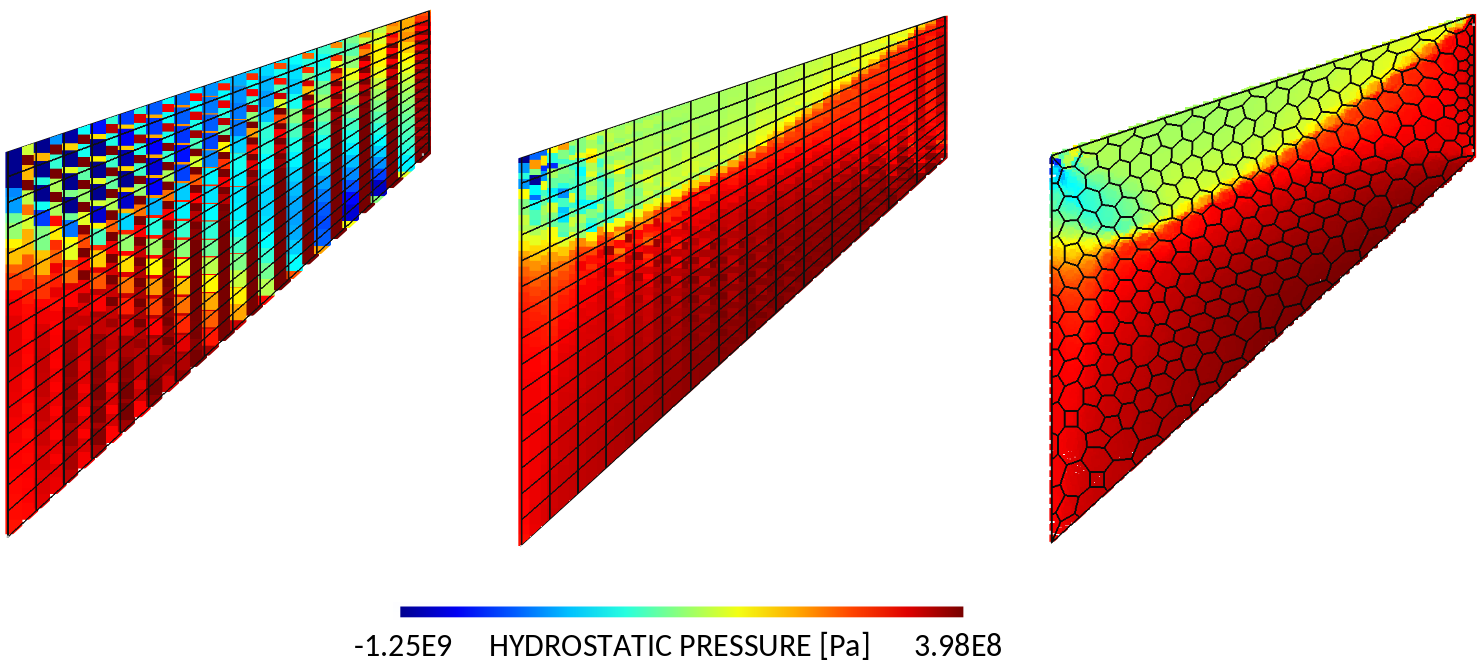
\includegraphics[width=12.cm]{../chapter_01_hho_mechanics/figures/cook_comp.png}
    \caption{Hydrostatic pressure map one the reference configuration at the limit load}
    \label{fig_cook}
\end{figure}

% ---------------------------------------------------------
% PARAGRAPH
% ---------------------------------------------------------
\paragraph{Numerical results}

As expected, the linear and quadratic finite element methods display respectively strong and mild oscillations of the pressure, whereas the HHO one shows no sign of locking.

% ---------------------------------------------------------
% -- SUBSECTION
% ---------------------------------------------------------
\subsection{Indentation test case}

% ---------------------------------------------------------
% PARAGRAPH
% ---------------------------------------------------------
\paragraph{Specimen and loading}

The last test case consists in the indentation of a cube of size $10$ mm. A pressure of $300$ MPa is imposed on the top surface see Figure \ref{fig_cube}).

% ---------------------------------------------------------
% PARAGRAPH
% ---------------------------------------------------------
\paragraph{Material}

The same perfect plastic material as that in \ref{sec_swelling_sphere} is considered for the present test case.

\begin{figure}[H]
    \centering
    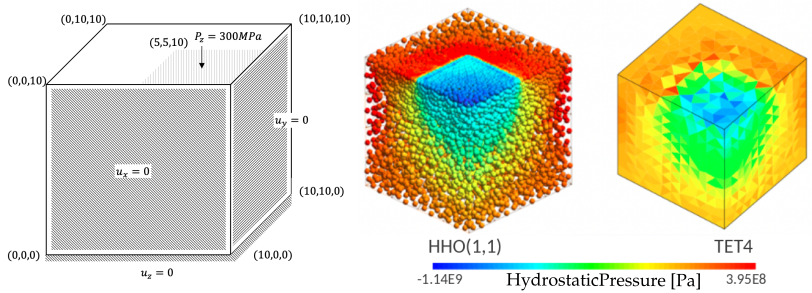
\includegraphics[width=12.cm]{../chapter_01_hho_mechanics/figures/cube.png}
    \caption{Hydrostatic pressure map one the reference configuration at the limit load}
    \label{fig_cube}
\end{figure}

% ---------------------------------------------------------
% PARAGRAPH
% ---------------------------------------------------------
\paragraph{Numerical results}

The pressure map at the end of the computation is displayed in Figure \ref{fig_cube}, and no sign of volumetric locking are present on the HHO computation, as opposed to the linear finite element one.